\section{Implementering}
\subsection{Control (Styring)}
I Simpel Snake er der ikke brug for nogen menu, og det er derfor muligt at holde styringen af spillet meget simpelt. Ved at definere de fire piletaster i \textit{Control}-klassen, en funktion til at sikre at der ikke bevæges i modsat retning, samt en funktion der gør det muligt at bevæge sig som en torrus og "gå igennem vægge og om på den anden side af verden", er alle styringkrav til Simpel Snake opfyldt. Resten af spillet håndteres da i model-koden.

\textit{Control}-klassen har metoden \textit{keyPressed}, som kommer af at \textit{Control}-klassen implementerer \textit{KeyListener}, som kaldes hver gang der tastes på tastaturet. Hvis tasten er en af de fire piletaster, kaldes funktionen \textit{move} i \textit{Snake}-klassen, der flytter hovedet i samme retning som piletasten.
Enum-klassen \textit{Direction} indholder \textit{RIGHT, LEFT, UP} og \textit{DOWN}. Dette bruges i \textit{Control}-klassen, da det ikke skal være muligt at bevæge sig i modsatte retning af slangens nuværende retning.
I \textit{Control}-klassens constructor er Direction som udgangspunkt sat til \textit{LEFT}, da slangen starter mod venstre. Hver gang der tastes på piletasterne, sikrer \textit{keyPressed}-metoden, at retningen ikke er modsat af den nuværende retning. Herefter flyttes slangen, uanset om den er midt på spillepladen eller om den bevæger sig rundt om torussen. Til sidst sættes \textit{Direction} til den nuværende retning, så det ved næste tasteanslag igen kan undersøges, at retningen ikke er modsat.


\subsection{Model}
Spillets model består af en række klasser, der tilsammen udgør selve spillets funktioner og objekter.
Klassen \textit{Field} bruges til at definere et et punkt, som repræsenterer et felt i banen. Den fungerer på samme måde som \textit{Point}-objekt-klassen, hvor koordinatsystemet starter oppe i venstre hjørne. Forskellen mellem \textit{Point}- og \textit{Field}-klassen, er hvordan man kommer frem til et punkt. \textit{Point}-klassen går først ud ad x-aksen og derefter ned ad y-aksen, hvorimod \textit{Field}-klassen gør det i omvendt rækkefølge. Da hele spillepladen er delt op i rækker og kolonner, frem for en x- og y-akse, er \textit{Field} lettere at bruge for at undgå forvirring, da to-dimensionelle arrays også er opdelt i rækker og kolonner, hvor den første værdi repræsenterer rækker, mens den anden værdi repræsenterer kolonner.

Funktionenen \textit{equals} er defineret i denne klasse, og bruges til at undersøge om to objekter ligger på samme felt, f.eks. slangens hoved og æblet. Æblet bliver oprettet i klassen \textit{Game}, hvor datafeltet \textit{position} afgør dets nuværende position.

Vi har valgt, at oprette spillepladen i \textit{Game}-klassen og ikke have en klasse, der kun beskriver banen for sig selv. Derved er de forskellige spilelementer defineret i deres egne klasser, så f.eks. \textit{Food} er en klasse for sig selv, \textit{Snake} er en klasse for sig selv i stedet for at være objekter i \textit{Game}. Hver klasse har de funktioner, der er relevante for dem, f.eks. \textit{getPosition} for at give deres nuværende position. 

Slangen selv er defineret i klassen \textit{Snake}. Slangens krop består af en række felter, hvoraf det første er hovedet, og de resterende er kroppen inklusiv halen til sidst. Koordinaterne for disse felter er gemt som elementer i en ArrayList kaldet \textit{positions}. Det første element er slangens første led, hovedet, det andet element er slangens andet led osv. Når et nyt led tilføjes, tilføjes et nyt element til listen. Dette sker, når slangen spiser et æble, hvor den ikke bevæger sig som ellers. I stedet tilføjes et nyt hoved på æblets felt. Hovedets retning er den samme, som slangens sidste bevægelse.

I \textit{Snake}-constructoren bliver slangens hoved og hale oprettet, hvor hovedet bliver placeret i banens centrum. Halen placeres i kolonnen til højre for på samme række.

I \textit{move}-metoden benyttes Action-klassen, der er oprettet som en enum, og betegner slangens handlinger: om slangen spiser et æble, er død eller bevæger sig (hhv. \textit{EAT, KILL, MOVE}). I \textit{move}-metoden undersøges der, om der er mad på samme felt som hovedets nye placering. Er dette tilfældet, bliver Action-statementet til \textit{EAT}. Hvis ikke, undersøges der om den nye placering for hovedet allerede indeholder slangens krop. Gør der det, bliver Action-statementet til \textit{KILL}. Hvis ikke, flyttes slangens hoved til den nye position. Resten af slangens krop følger med ved at ændre koordinaterne i \textit{positions} fra halen og op til hovedet, dvs. at halens koordinater bliver næstsidste led, næstsidste bliver tredjesidste osv. Slangens krop flyttes først, hvorefter hovedet flyttes til sidst, for at undgå at andet led indtager samme plads som hovedet.

I \textit{Game}-klassen findes \textit{checkAction}-metoden, der undersøger om slangen spiser eller dør. Hvis Action-statementet er \textit{EAT}, øges slangens længde ved at tilføje et nyt element på æblets felt, som fungere som nyt hoved. Scoren inkrementeres, der laves et nyt æble, og Action-statementet sættes til \textit{MOVE}.
Hvis Action-statementet er \textit{KILL}, nulstilles scoren, og spillet slutter ved at slangen ikke længere kan bevæge sig.
Herudover findes \textit{generateFood}-metoden, som sikrer, at maden altid placeres på et gyldigt felt, dvs. et felt der ikke er udfyldt af slangen. For at sikre dette, placeres æblet på et tilfældigt felt inden for banens rammer, hvorefter der undersøges om et af slangens led har samme koordinater som æblets felt. Er dette tilfældet, gives æblet et nyt felt, indtil det lander på et felt uden slangen. Er slangen tilpas stor, er dette dog ikke effektivt, da der er stor sandsynlighed for at ramme et felt, der er optaget af slangen. Af denne årsag undersøger metoden først, om slangen fylder mere end halvdelen af banen. Er dette tilfældet, laves der i stedet en liste med alle tomme felter vha. en indlejret for-løkke, der løber gennem alle række og kolonner, hvorefter et tilfældigt element i listen vælges som æblets position.

De fire klasser \textit{Food, Score, Game} og \textit{Snake} nedarver fra klassen \textit{Observable}, så det er muligt for View at modtage ændringerne i \textit{Model}, uden at \textit{Model} afhænger af View.


\subsection{View (Brugergrænseflade)}
Brugerfladen er samlet i klassen \textit{GameView} der forlænger \textit{JFrame}. I \textit{GameView} findes kun en constructor, hvor der oprettes et \textit{ScorePanel}-objekt, der placeres øverst i vinduet, og et \textit{BoardPanel} objekt, der placeres direkte under det. Board-panelet viser selve banen med slangen og æblet, der begge er vist ved farvede firkanter. 

\textit{ScorePanel}-klassen forlænger \textit{JPanel} og implementerer \textit{Observer}. Klassen har en \textit{update}-metode, der gentegner, hver gang noget ændrer sig i de klasser i model-pakken, der forlænger \textit{Observable}. 
\textit{paintComponent}-metoden benyttes til at tegne score-teksten. Selve panelet oprettes i constructoren.

\textit{BoardPanel} forlænger også \textit{JPanel} og implementerer \textit{Observer}, for at den også kan registerere ændringer i model-klasserne. \textit{BoardPanel} består af en række draw-metoder, samt en \textit{paintComponent}-metode, der kalder på draw-metoderne for at tegne alle spillets komponenter på spillets bane og spillets bane selv.
I \textit{drawSnake}-metoden bruges positionerne for slangens felter til at tegne slangen. Størrelsen for et felt udregnes i \textit{getWindowRectangle}-metoden, og afhænger af vinduets størrelse og antallet af banens felter. Når feltets størrelse er udregnet, tegnes en rektangel med feltets størrelse på alle felterne i slangens positions-ArrayList.

Da spillepladen skal være mellem 5x5 og 100x100 felter, kan det skabe problemer, hvis man ikke kan justere størrelsen på vinduet. Vinduet kan være for stort til at passe på en gennemsnitlig computerskærm. Det er derfor nødvendigt at gøre spillets vinduestørrelse fleksibel. En løsning på dette problem ville være at bestemme en fast størrelse for felterne, og lade vinduet justere sin størrelse efter dette. Ulempen ved metoden er, at store baner kan blive for store til at være på en normal skærm. Derfor har vi valgt at lave en fleksibel størrelse for felterne, så de følger forholdet mellem vinduestørrelse og antal felter.
I figur \ref{fig:windowsize} kan man se, at hvis vinduet skal være justerbart, så kan man risikere at selve banen bliver aflang og ikke særlig pæn at spille på.

\begin{figure}[h]
	\centering
	\graphicspath{ {pics/} }
	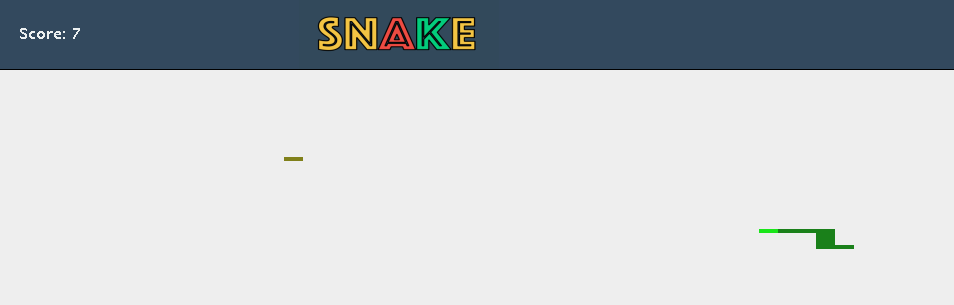
\includegraphics[width=0.8\textwidth]{WindowSize.png}
	\label{fig:windowsize}
	\caption{Exemple på udstræktede felter.}
\end{figure}
